\documentclass[
  11pt,
  letterpaper,
   addpoints,
  % answers
  ]{exam}

\usepackage{../exercise-preamble}
\usepackage{multicol}
\begin{document}

\noindent
\begin{minipage}{0.47\textwidth}

\includegraphics[width=\textwidth]{../fcfm_die}
\end{minipage}
\begin{minipage}{0.53\textwidth}
    
\begin{center} 
\large\textbf{Análisis y Diseño de Circuitos Eléctricos} (EL3101-2) \\
\large\textbf{Tarea 3} \\
\normalsize Prof.~Santiago Bradford V.\\
\normalsize Prof.~Aux.~Erik Saez A. - Rodrigo Catalán\\
             - Byron Castro R.
\end{center}
\end{minipage}

\vspace{0.5cm}
\noindent
\vspace{.85cm}

\fbox{%
  \begin{minipage}{0.95\linewidth}
    \textbf{Obs:} Recuerde que solo serán revisadas tres preguntas al azar. No olvide explicar de forma clara y precisa su desarrollo. \\\\
    \textbf{Fecha de entrega}: 29 de Junio
    
  \end{minipage}
}

\begin{questions}
    %%%%%%%%%%%%%%%%%%%%%%%%%%%%
    \question Un filtro suprime banda implementado mediante OPAMPs se muestra en la Figura~\ref{fig:suprime-banda}. Determine \( H(s) = \frac{V_o}{V_i(s)} \) suponiendo que los OPAMPs son ideales.
     
\begin{figure}[h!]
    \centering
    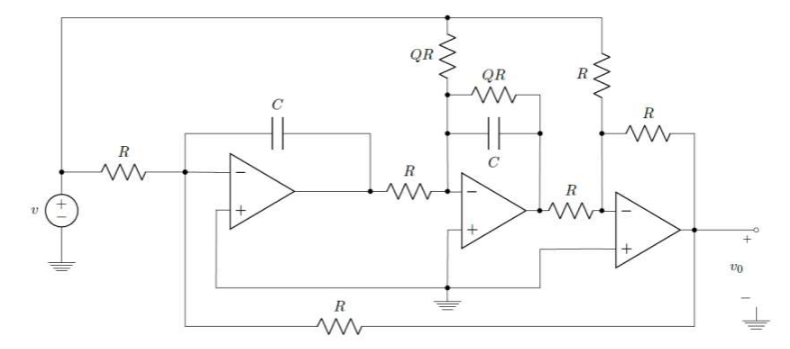
\includegraphics[width=0.6\textwidth]{Tarea_3_1}
    \caption{Esquema del problema}
    \label{fig:suprime-banda}
\end{figure}

%%%%%%%%%%%%%%%%%%%%%%%%%%%
    \question   Para el circuito OPAMP de la Figura~\ref{fig:tarea3-2}, determine la función de transferencia \( H(s) = \frac{V_{o2}(s)}{V_i(s)} \) usando directamente impedancias o admitancias en Laplace. Escriba \( H(s) \) en la forma estándar, donde la función está factorizada en polos y ceros y se computa la ganancia \( K \).

\underline{Nota:} Determine primero \( H_1(s) = \frac{V_{o1}(s)}{V_{i}(s)} \) y luego \( H_2(s) = \frac{V_{o2}(s)}{V_{o1}(s)} \).

\begin{figure}[h!]
    \centering
    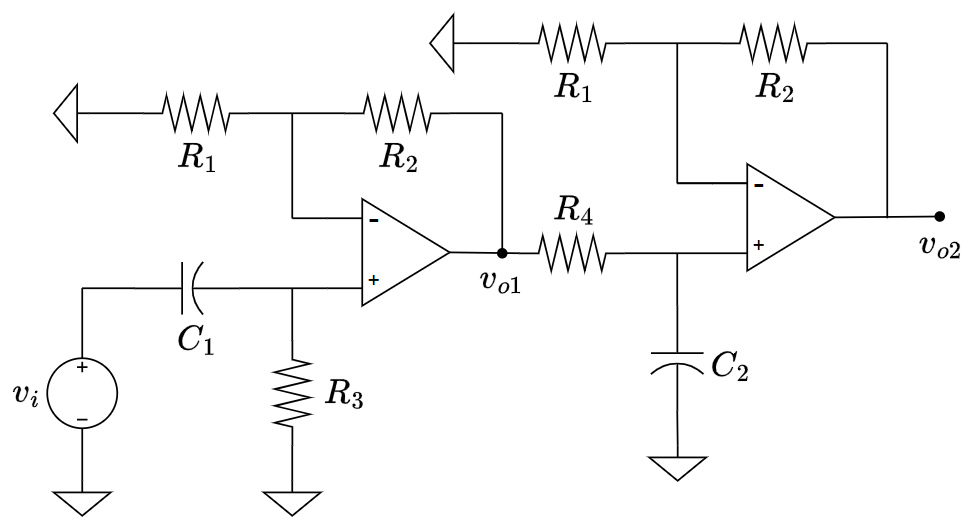
\includegraphics[width=0.5\textwidth]{Tarea_3_2}
    \caption{Esquema del problema}
    \label{fig:tarea3-2}
\end{figure}
%%%%%%%%%%%%%%%%%%%%%%%%%%%
\question   La respuesta al escalón unitario de un circuito lineal-invariante está dada por:
    $$s(t) = 1000[e^{-200t} + 2e^{-2000t}], 
    \hspace{0.5cm}t>0$$
    \begin{enumerate}
        \item Determine la función de transferencia $H(s)\triangleq \mathcal{L}\{h(t)\}$, dejando expresados los polos y ceros $(s+\omega_0)$ de la forma $\omega_0(1+s/\omega_0)$.
        \item Analice por separado las asíntotas de cada término de $20\log|H(j\omega)|$ y represéntelas gráficamente. Luego, dibuje el diagrama de Bode asintótico de magnitud para $|H(j\omega)|$, indicando claramente las frecuencias de corte, pendientes y ganancias.
    \end{enumerate}
%%%%%%%%%%%%%%%%%%%%%%%%%%%
\question Considere la Figura~\ref{fig:tarea3-3} que muestra uno de los canales de un amplificador de audio que se requiere conectar a dos parlantes, uno que transmita las altas frecuencias y otro las bajas frecuencias. El objetivo de este problema es comprender la utilidad de los circuitos RL y RC como filtros de frecuencia. Para ello se solicita:

\begin{enumerate}
    \item Suponga el bloque del canal de amplificador de audio como una fuente $V_{in}$ y los parlantes como resistencias. Luego, dibuje el circuito.
    
    \item Sea $V_1$ y $V_2$ los voltajes asociados a $S_1$ y $S_2$ respectivamente. Para cada uno de ellos, determine su función de transferencia y señale qué tipo de filtrado realiza cada función de transferencia.
    
    \item Investigue en los apuntes del curso sobre los valores típicos de $R$, $C$ y $L$. Escoja el valor que más le acomode y dibuje el diagrama de Bode en un solo gráfico para cada función de transferencia.
    
    \item En base al diagrama anterior, ¿sus valores escogidos son adecuados? Justifique por qué sí o por qué no. Explique en base al sonido que escuchará por el equipo de audio.
\end{enumerate}

\begin{figure}[h!]
    \centering
    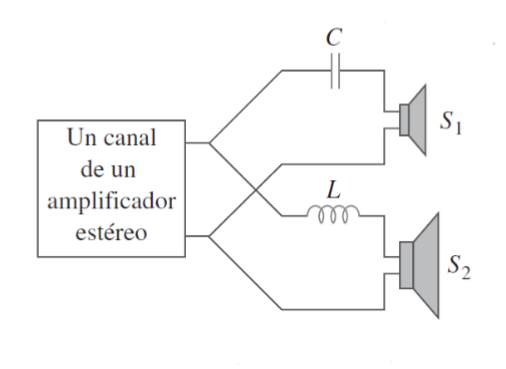
\includegraphics[width=0.5\textwidth]{Tarea_3_3}
    \caption{Esquema del problema}
    \label{fig:tarea3-3}
\end{figure}
\newpage
%%%%%%%%%%%%%%%%%%%%%%%%%%%%%

\question   
 \begin{enumerate}
    \item Dado el diagrama de Bode de magnitud de la Figura~\ref{fig:bode}, determine la función de red $H(s)$.

    \begin{figure}[h!]
        \centering
        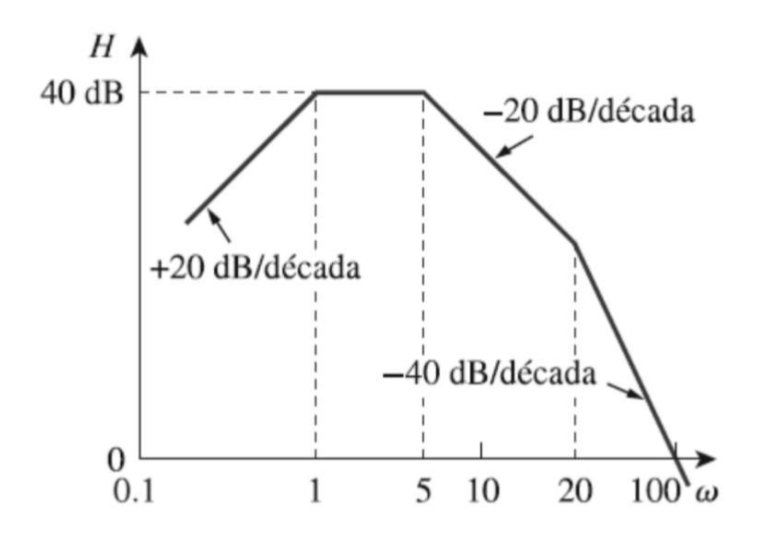
\includegraphics[width=0.5\textwidth]{Tarea_3_4}
        \caption{Diagrama de Bode.}
        \label{fig:bode}
    \end{figure}

    \item Dibuje los diagramas de Bode de magnitud y fase para la función de transferencia:
    \begin{equation}
        H(s) = \frac{10s(s + 20)}{(s + 1)(s^2 + 60s + 400)}
        \label{eq:bode-func}
    \end{equation}
\end{enumerate}

%%%%%%%%%%%%%%%%%%%%%%%%%%%
\question El \textit{switch} $S_1$ del circuito de la Figura~\ref{fig:circuito5} ha estado cerrado durante un largo período de tiempo y se abre en $t = 0$. Por otra parte, el \textit{switch} $S_2$ ha estado abierto durante un largo período de tiempo, cerrándose en $t = 0$, al mismo tiempo que se abre $S_1$.

\begin{figure}[h!]
    \centering
    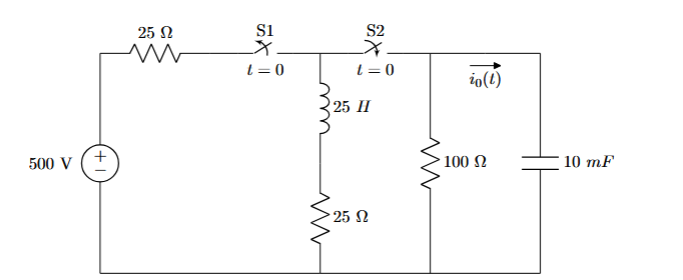
\includegraphics[width=0.65\textwidth]{Tarea_3_5}
    \caption{Circuito Propuesto 5}
    \label{fig:circuito5}
\end{figure}

\begin{enumerate}
    \item[a)] Plantear el circuito con el método de mallas para $t > 0$ en el dominio de Laplace.
    \item[b)] Determinar $I_0(s) = \mathcal{L}[i_0(t)](s)$.
    \item[c)] Calcular $i_0(t)$ para $t \geq 0$.
\end{enumerate}

%%%%%%%%%%%%%%%%%%%%%%%%%%%
\end{questions}
\end{document}